% !TEX root = ../../../main.tex
% 来源：中学数学实验教材·第三册（高中数学）
% 章节：二次函数 / 二次函数
% 原始文件：5.tex，行 926-941
% 类型：tikz
% ---
    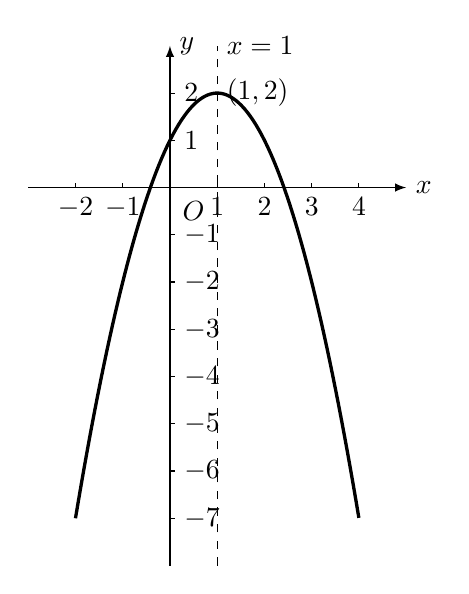
\begin{tikzpicture}[>=latex, scale=.6]
 \draw[->] (-3,0)--(5,0)node[right]{$x$};
\draw[->] (0,-8)--(0,3)node[right]{$y$};
\foreach \x in {-2,-1,1,2,3,4}
{
    \draw (\x,0)node[below]{$\x$}--(\x,.1);
}
\foreach \y in {-1,-2,...,-7,1,2}
{
    \draw (0,\y)--(.1,\y)node[right]{$\y$};
}
\node at (.5,-.5){$O$};          
\draw[dashed] (1,-8)--(1,3)node[right]{$x=1$};
\draw [domain=-2:4, samples=100, very thick]plot(\x, {-(\x-1)*(\x-1)+2});
\node at (1,2)[right]{$(1,2)$};
    \end{tikzpicture}
